

\section{Reactor Deployment}
 
\subsubsection{Valuing Small Modular Reactor Deployment using Real Options}

One of the major difficulties holding back the adoption of Nuclear Power Plants is the large upfront capital costs required to begin construction on a new plant.  Small Modular Reactors offer a solution to this problem, with the ability to build a cluster of reactors in phases, significantly reducing the initial upfront capital required and thus reducing the risk of the project.  Since the construction will be done in phases, there will be options available during the construction such as abandonment due to unfavorable market conditions.  Using a framework for valuing real options, this paper will quantify value in projects that deploy modular reactors in phases that is currently excluded in traditional present worth calculations.     

\subsection{Valuing Small Modular Reactor Deployment}

In a traditional present worth calculation for reactor deployment, it is assumed that regardless of the outcome of the first phase of construction, the second phase will go forward.  However, this decision will not be made now, but in the future based off of future market conditions, and in particular how much the first phase of the project is worth.  For example, if the first phase of the project has a negative present worth, the second phase of construction will be abandoned.

First, an explanation of a real option will be given and then the framework to value these options.  As this work steps through the framework, an example of an application to an Independent Power Producer will be developed, with a project in Tennessee Valley Authorities’ district in which 6 B W mPower reactors are to be deployed.      

\subsection{Real Options}

A real option is the right, but not the obligation, to take an action at a predetermined cost called the exercise price, for a predetermined period of time – the life of the option [1]. This is related to financial options, except is an option on a business decision about a capital investment, versus a financial underlying such as stock price.   

The framework for valuing real options is broken into four parts.  First, the base case present worth calculation must be conducted.  Then, model the uncertainties involved in this calculation, which will be consolidated into one uncertainty, the rate of return on the project.  Once this has been done, a lattice of the underlying can be made, which incorporates the growing uncertainty over time of the value of the project.  The actual outcome of the project will be one path through this lattice.  Now, the possible future outcomes are known and managerial flexibilities can be added.  Finally, the future outcomes, with flexibilities included, can be valued and discounted back to time 0 to find the present worth of these options, and thus the project. 

\subsection{Traditional Present Worth Calculation}

\subsubsection{Busbar Cost of Electricity}

The equation below is used to calculate the busbar cost of electricity, that is, the cost to build the generating asset amortized over all of the electricity it will produce throughout its life.  The LHS of the equation is the present worth of the stream of income from electricity generation and the RHS is the upfront capital cost and the present worth of the stream of costs for O M and fuel [2].  
\begin{equation}
	\sum \frac{8.766 K L_i e}{ (1+x)^i }  =
		\sum \frac{ \phi_i I_0}{ (1+x)^i } +
		\sum \frac{ O_i }{ (1+x)^i } +
		\sum \frac{ F_i }{ (1+x)^i }
\end{equation}

\subsubsection{Independent Power Producers}

Historically, utilities have been vertically integrated through the electrical generation industry.  They expand generation as needed based on demand, and when building a new plant, will try to minimize the busbar cost of electricity of the plant.  However, the industry has begun restructuring how it operates and Independent Power Producers (IPP) now they play a bigger role.  An Independent Power Producer owns and operates electrical generation assets and sells this power to a wholesale electrical market [3].  These companies are driven by market forces, and thus provide a better foundation for the methods used in analyzing real options.  An IPP is interested in maximizing the present worth (ideally profit) from any project it undertakes.    

\begin{equation}
	NPV = \sum \frac{8.766 K L_i e}{ (1+x)^i }  -
		\sum \frac{ \phi_i I_0}{ (1+x)^i } -
		\sum \frac{ O_i }{ (1+x)^i } -
		\sum \frac{ F_i }{ (1+x)^i }
\end{equation}

\subsubsection{B W mPower Reactor}

In order to calculate the present worth of one mPower reactor, several parameters are needed.  These parameters include upfront capital costs, operation and maintenance costs (O M), fuel costs and reload schedule, a capital structure, and a sale price for electricity.  Using the given parameters, a present worth of around \$12 million was found.  This present worth is associated with a rate of return of around 10.2\%, which is higher than the effective discount rate of 9.4\%, signifying it will most likely be a good project.

\subsection{Value of Real Options}
\subsubsection{Consolidating Uncertainty into the Rate of Return}

In order to build a lattice of the underlying, all of the uncertainties of the project can be consolidated into one uncertainty, the rate of return of the project [3].  Using the Microsoft Excel add-on  $@$Risk, the uncertainties in Table II of Appendix B were modeled for the mPower reactor.  Then, using Monte Carlo simulation with 1000 trials, the standard deviation of rate of return was found to be 28.5.  The larger the value of the standard deviation, the faster the uncertainty grows as the project progresses through time, and thus the more valuable managerial options are in the future.  

\subsubsection{Value of Underlying Project}

Once the standard deviation is found, a lattice of the underlying is built.  This represents the possible future outcomes that this project could take.  The lattice is developed as a random walk of the value of the project throughout time.  The justification for this approach was a result of a proof by Samuelson in 1965.  He was able to prove that properly anticipated prices fluctuate randomly [4].  Since an IPP operates in a real market, it is not unreasonable to assume that the company will value the project as well as possible and have close to complete information.  \\

In order to build the lattice, a risk-free interest rate is needed.  This is the rate at which money is expected to grow, with no risk of losses.  Typically, treasury bonds are used to represent this risk-free rate.  One main assumption that these methods are built upon is that the market has no arbitrage opportunities.  Due to this assumption, the expected value of the project grows at the risk-free interest rate.  If this was not so and the expected growth rate of the project was larger, everyone would take money at the risk-free interest rate and invest in this project, which on average returns more.  \\

The lattice can be developed as a geometric process or an additive process.  The lattice is constructed for a given time frame, $T$, and then divided into $N$ periods.  As $N \rightarrow \infty$, the geometric process approaches a lognormal distribution, while the additive process approaches a normal distribution.  The geometric process is typically used to model things such as stock prices, where it is known that the value will never be below 0.  In the case of the B \& W reactor, it is possible that the value of the project will drop below 0, so an additive process will be used to model the underlying uncertainty.

\begin{figure}
\centering
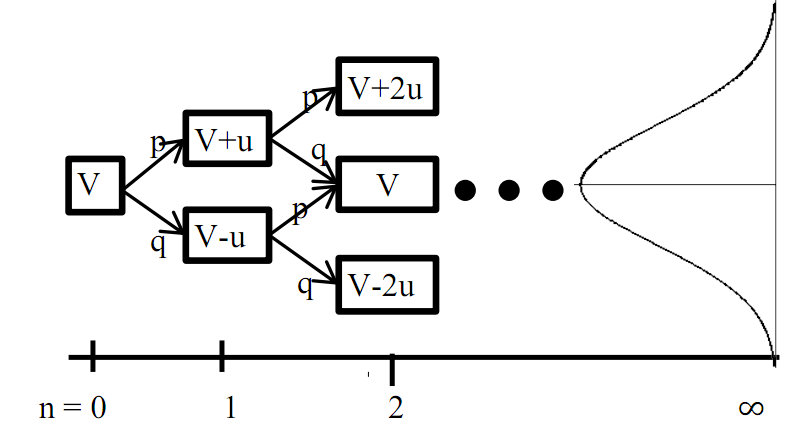
\includegraphics[width=3.5in]{reactor_underlying_lattice}
\caption{ Examply of underlying additive process  }
\end{figure}

The underlying lattice will model the sample paths possible as the value of one reactor undergoes a random walk throughout the 2 years of construction.  The lattice used for this work will divide the time frame into 7 periods, which provides enough resolution of the possible future outcomes.  The formulas to construct a lattice are located in Appendix A, the parameters used to construct the lattice are located in Appendix B, Table II, and the final lattices are located in Appendix D.

\subsection{Project Flexibility}

\begin{figure}
\centering
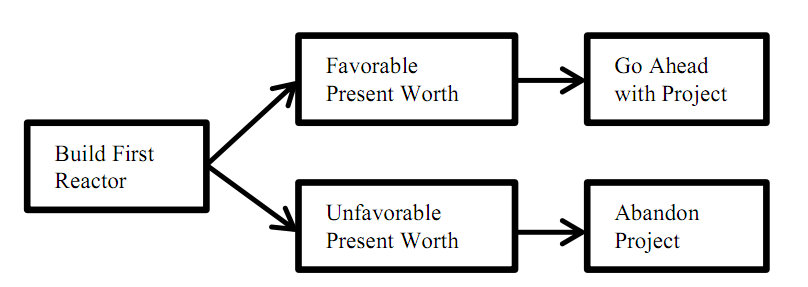
\includegraphics[width=3.5in]{reactor_event_tree}
\caption{Event tree of project flexibility}
\end{figure}

Now that the possible outcomes of the value of one reactor are known, managerial flexibility can be added to the project and the outcomes in each final state can be developed.  The first reactor can be seen as a market test for the value of each reactor in the cluster.  Once the value of a single reactor is known at year 2, it is assumed that management will make the decision either to abandon the project if the present worth of 1 reactor is unfavorable, or go ahead with the project and build 5 more reactors over the next 10 years if the present worth is favorable.    



  In order to find the present worth of a cluster of reactors, the following factor can be used.
\begin{equation}
\xi = 1 + (\frac{P}{F},r,2)  + (\frac{P}{F},r,4)  + (\frac{P}{F},r,6)  + (\frac{P}{F},r,8)  + (\frac{P}{F},r,10)
\end{equation}
For the given effective discount rate, This calculation assumes that each plant has a 2 year construction period and 6 reactors will be built consecutively.  Finally, the present worth of a cluster of 6 reactors can be found to be \%48 million.

In terms of the value ($V$) of the project at time 2, management can incur the strike price ($S$) of expansion to obtain a value of $\xi V - S$, where $\xi$ is defined in equation (), or abandon future construction and keep the current value $V$.  The strike price could be the costs associated with expanding the license with the NRC and changes to the building structure for the extra 5 reactors.
\begin{equation}
V_{i,d}^\prime = \mbox{ max } \left\{	\xi V_{i,d} - S  , V_{i,d}      
				\right\}		
			\mbox{ for } i=N
\end{equation}
Once the outcomes in the final states are known, the value can be discounted back to time 0 using risk-neutral probabilities and the risk-free discount factor.  Once a single value for the project is found for time 0, this can be compared to the project without flexibility.  That is, the value of the project in which regardless of the value of the first reactor, 5 more reactors are built.

\subsection{Results}

In order to find the value of the managerial option to abandon the project, the value of the project with and without flexibility was determined.  In the case that the project will go ahead regardless of market conditions, the project is worth around \$20.9 million.  When given flexibility for the decision based on future market conditions, the project is worth around \$23.2 million.  In conclusion, the value of flexibility for this project is around \$2.3 million.  Not only is there less upfront capital needed for this type of reactor deployment, there are also valuable options available to management in order to take advantage of the given market conditions at any given time.





\subsection{Reactor Appendix}
\subsubsection{Equations - Present Worth}

Fixed charge rate for given capital structure, tax rate, and depreciation scheme
\begin{equation}
	\phi_i = \pi + d_i + r \left[  1 - \sum_j d_j   
				\right]
			+ \frac{\tau}{1-\tau}
				\left[  r_s f_s (1- \sum_j d_j) + d_i - d_i^\prime
				\right]
\end{equation}

Effective discount factor for a given capital structure, including taxes
\begin{equation}
x = r_b f_b (1-\tau)  + r_s f_s
\end{equation}

Rate of return for the project

In order to find the rate of return for the project, all of the cash flows are consolidated into present worth at time period one with the company’s effective discount rate.  This is then compared to the initial capital expenditure for the project.
\begin{equation}
ror = ln (  \frac{ NPV_{t=1} }{CAPEX} )
\end{equation}


\subsubsection{Equations - Lattice Construction}

Time step for lattice
\begin{equation}
\delta_t = \frac{T}{N}
\end{equation}

Risk-free interest factor per period
\begin{equation}
R_i = exp( r_f \delta_t )
\end{equation}

Risk-free discount factor per period
\begin{equation}
R_d = \frac{1}{R_i}
\end{equation}
Up factor for lattice
\begin{equation}
U = V_0 \left[	exp( \delta_t \sqrt{ \sigma } ) - 1
	  \right]
\end{equation}

Risk-neutral up probabilities
\begin{equation}
p_u = \frac{   V_0 (1-R_i) + U    }{  2 U          }
\end{equation}

Risk-neutral down probability
\begin{equation}
p_d = 1-p_u
\end{equation}

State value for lattice
\begin{equation}
V_{i,d} = V_0 + iU - 2dU
\end{equation}

State probability for lattice
\begin{equation}
P_{i,d} = p_u P_{i-1,d} + p_d P_{i-1,d-1}
\end{equation}


State values for project
\begin{equation}
V_{i-1,d}^\prime = R_d (p_u V_{i,d}^\prime + p_d V_{i,d-1}^\prime
\end{equation}
Once the outcomes are known for each possible final 
state, the values can be discounted back to time 0

\subsubsection{Input Data}

B \& W reactor present worth calculation
\begin{center}
\begin{table}
\caption{ B \& W Reactor Parameters}
\centering
\begin{tabular}{ | l |  l |}
\hline
Parameter &	Value  \\
\hline
$I_0$		&	\$325 million	\\
$O_i$		&	\$ 12.5 million	\\
$F_i$		&	\$ 27 million	\\
$t_f$		&	5 years	\\
$e_i$		&	53.5 $\frac{mills}{kWh}$	\\
$L_i$		&	90 \%	\\
$C$		&	125 MW	\\
$T$		&	60 years	\\
$f_b$		&	50 \%	\\
$r_b$		&	8 \%	\\
$f_s$		&	50 \%	\\
$r_s$		&	14 \%	\\
$\tau$		&	40 \%	\\
$d_i, d_i^\prime$	&	$\frac{1}{40}$	\\
\hline
\end{tabular}
\end{table}
\end{center}

Uncertainty Distributions 

The following figures show the input distributions for the Monte Carlo simulation.

\begin{figure}
\centering
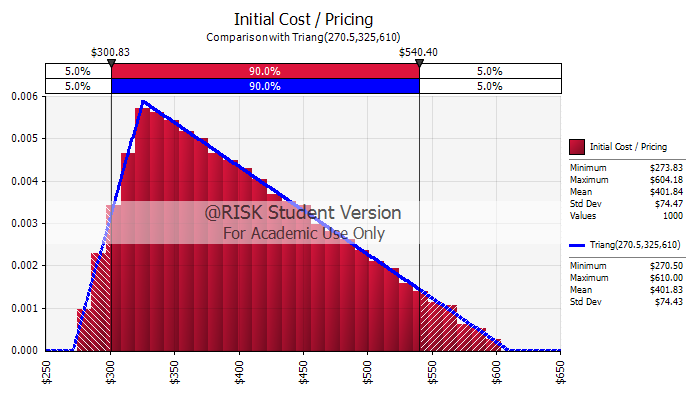
\includegraphics[width=4in]{reactor_upfront_capex}
\caption{Upfront Capital Expenditure Distribution}
\end{figure}

\begin{figure}
\centering
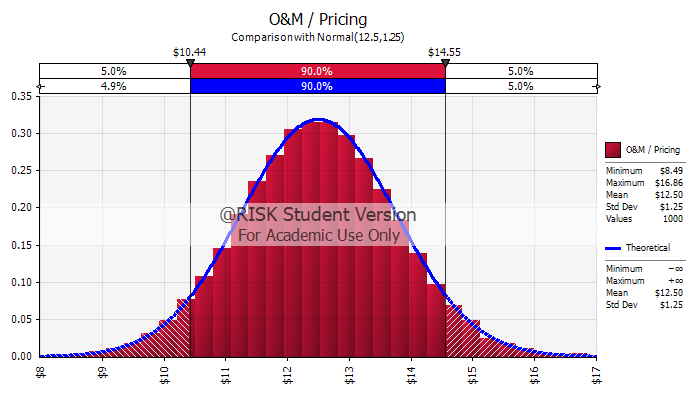
\includegraphics[width=4in]{reactor_o_and_m}
\caption{ O \& M Cost Distribution   }
\end{figure}
 
\begin{figure}
\centering
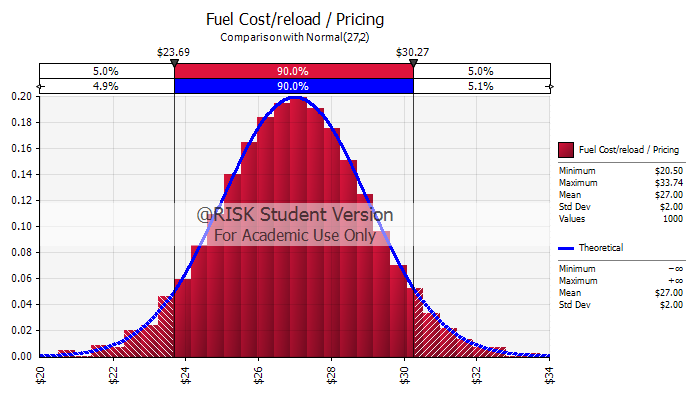
\includegraphics[width=4in]{reactor_fuel_cost}
\caption{ Fuel Cost Distribution per Reload   }
\end{figure}

\begin{figure}
\centering
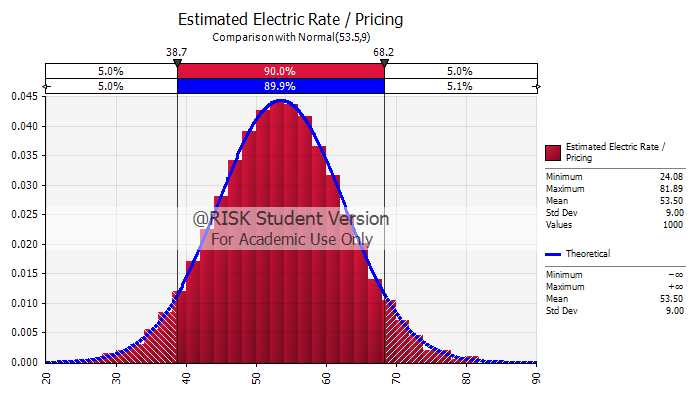
\includegraphics[width=4in]{reactor_sale_price}
\caption{ Sale Price of Electricity Distribution   }
\end{figure}

\begin{center}
\begin{table}
\caption{Lattice Parameters}
\centering
\begin{tabular}{ |  l  |  l  | }
\hline
Parameter	&	Value	\\
\hline
$r_f$		&	3 \%	\\
$T$		&	2 years	\\
$N$		&	7 periods	\\
$\delta_t$		&	$\frac{2}{7}$ years	\\
$V_0$		&	\$ 12 million	\\
$S$		&	\$ 25 million	\\
$U$		&	\$ 1.94 million	\\
$p_u$		&	52.6 \%	\\
$p_d$		&	47.3 \%	\\
\hline
\end{tabular}
\end{table}
\end{center}



\subsubsection{Monte Carlo Output}

\begin{figure}
\centering
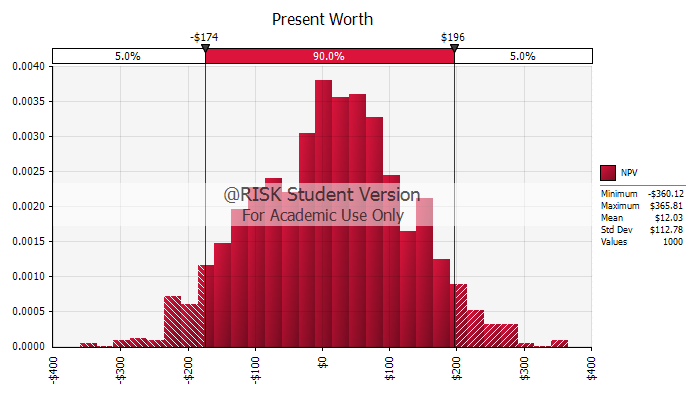
\includegraphics[width=4in]{reactor_present_worth}
\caption{ Present Worth Distribution   }
\end{figure}

\begin{figure}
\centering
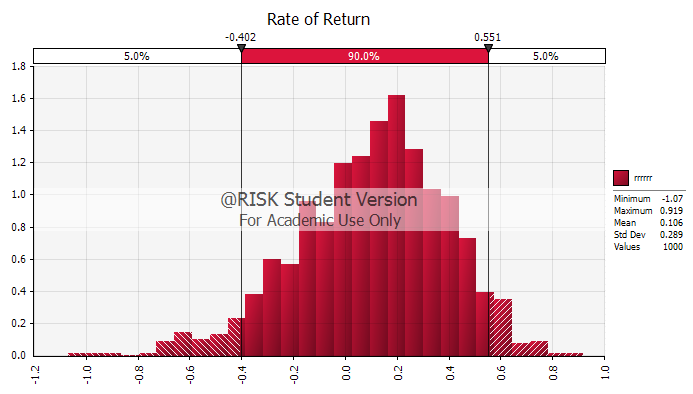
\includegraphics[width=4in]{reactor_ror}
\caption{ Rate of Return Distribution   }
\end{figure}
  
\subsubsection{Lattices}


\begin{figure}
\centering
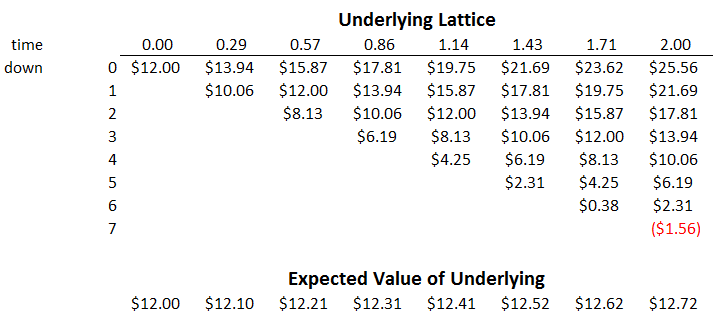
\includegraphics[width=4in]{reactor_lattice_single}
\caption{  State Values of Single Reactor Project  }
\end{figure}

\begin{figure}
\centering
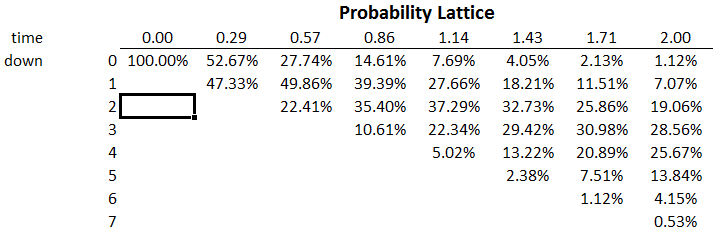
\includegraphics[width=4in]{reactor_lattice_probability}
\caption{  Probability of Given State for Single Reactor Project  }
\end{figure}

\begin{figure}
\centering
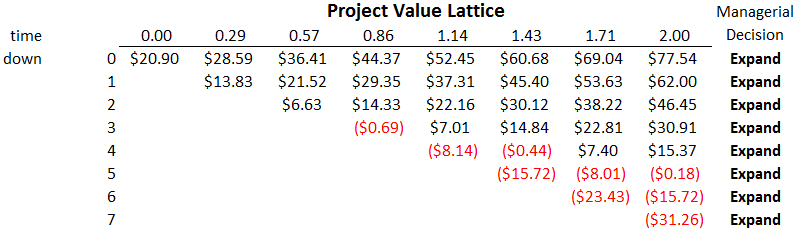
\includegraphics[width=4in]{reactor_lattice_cluster}
\caption{  State Values of Cluster of Reactors with no Flexibility  }
\end{figure} 


\begin{figure}
\centering
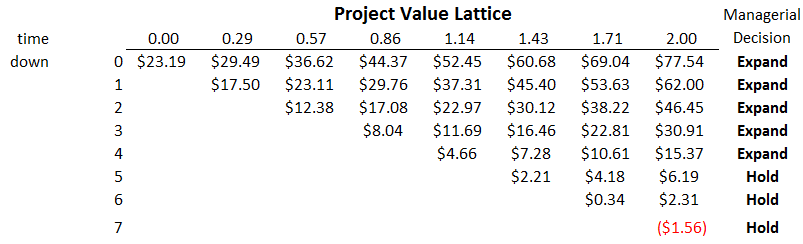
\includegraphics[width=4in]{reactor_lattice_cluster_flexibility}
\caption{  State Values of Cluster of Reactors with Flexibility  }
\end{figure}



\subsubsection{Nomenclature}

\begin{tabular}{ l l }
$I_0$ 	&	 Initial capital costs	\\
$O_i$ 	&	 O \& M costs for year \\
$F_i$	&	 Fuel costs for year i  \\
$t_f$	&	 Time between fuel reloads  \\
$C$	&	 Capacity of reactor  \\
$L_i$	&	 Capacity factor for year i   \\
$e_i$	&	Sale price of electricity for year i  \\
$T$	&	 Lifetime of reactor  \\
$PW_6$&	 Present worth of 6 B W reactor  \\
$PW_1$&	 Present worth of 1 B W reactor  \\
$\phi_i$	&	 Fixed charge rate  \\
$\pi $	&	 Property taxes and insurance  \\
$d_i$	&	 Book value depreciation fraction  \\
$d_i^\prime$	&	 Depreciation fraction for taxes  \\
$r_s$	&	 Rate of return for stock  \\
$f_s$	&	 Fraction stock  \\
$r_b$	&	 Rate of return for bonds  \\
$f_b$	&	 Fraction bonds  \\
$x$	&	 Effective discount factor   \\
$r_f$	&	 Risk-free interest rate  \\
$R_i$	&	 Risk-free interest factor  \\
$R_d$	&	 Risk-free discount factor  \\
$\sigma$	&	Standard deviation of rate of return  \\
$V_0$	&	 Initial present worth of reactor   \\
$V_{i,d}$ &	Value of lattice for time i and d down movements  \\
$P_{i,d}$ &	Probability of state for time i and d down movements   \\
$S$	&	 Strike price for expansion   \\
$N$	&	 Number of periods in lattice  \\
$\delta_t$	&	 Time step in lattice   \\
$U$ 	&	 Up factor for lattice   \\
$p_u$  &	 Risk neutral up probability   \\
$p_d $  &	 Risk neutral down probability   
\end{tabular}